
%*************************************************************************
%
%   SEE CALIBRATION_1 FOR THE FIRST PART (COMMENTED HEREAFTER)
%
%************************************************************************


%----------------------------------------------------------------------------------------
%	8./ Calibration
%----------------------------------------------------------------------------------------
%\section{Calibration}
%\label{se:calibration}

%We present the calibration of the absolute scale of the flux densities
%for the NIKA2 instrument in this section using Uranus as the main
%primary calibrator. Practically, at the stage of the FOV
%reconstruction (see Sect.~\ref{se:geometry}), an absolute
%coefficient factor per detectors is derived using a \bm\ scan of
%Uranus. This step realizes also the inter-calibration of all the KID,
%as the coefficient factors give the KID gains. Secondly, the flux
%density absolute scale is further refined by monitoring the primary
%calibrator all along the observation campaign to estimate an
%absolute calibration correction.

%We have evidenced a daily variation of the absolute calibration
%coefficients as a function of the observation date, which is related
%to temperature-induced variation of the beam size. If left uncorrected, this variation
%induces a sizable increase of the calibration uncertainties. To
%overcome this issue, we primarily flag the most impacted observation
%dates and exclude the observations acquired during these periods. This
%conservative approach constitutes the baseline calibration method,
%which is further used for the performance assessment. For cross-check,
%we also proposed an alternative method relying on a photometric
%correction depending on the beam size. Both approaches require an
%accurate monitoring of the beam size as a function of the observation
%date.


%First we describe the method for the absolute calibration in
%Sect.~\ref{se:calibration_method}, then we present the
%inter-calibration and the flat fields in
%Sect.~\ref{se:flat_field}. The temperature-induced variation and the
%beam size monitoring are then discussed in
%Sect.~\ref{se:beam_variation}. Finally, the baseline calibration is
%presented in Sect.~\ref{se:baseline_calibration} and the calibration
%with a photometric correction in
%Sect.~\ref{se:photometric_correction}.  



%---------------------------------------------------------------------
%	Method
%---------------------------------------------------------------------

%\subsection{Absolute calibration procedure and photometric system}
%\label{se:calibration_method}

%\subsubsection{Photometric system}
%\label{se:photometric_system}

%\subsubsection{Color correction}
%

%\subsubsection{Diffuse source}
%\label{se:extended_source_calib}

%\subsubsection{Practical calibration}
%

%---------------------------------------------------------------------
%	INTERCALIBRATION
%---------------------------------------------------------------------
%\subsection{Relative calibration \& flat fields}
%\label{se:flat_field}


%---------------------------------------------------------------------
%	TEMPERATURE-INDUCED VARIATION
%---------------------------------------------------------------------
%\subsection{Temperature-induced variations}
%\label{se:beam_variation}

%\subsubsection{Beam monitoring using bright source scans}
%\label{se:beam_monitoring_otf}

%\subsubsection{Beam monitoring using pointing}
%\label{se:beam_monitoring_pointing}


%---------------------------------------------------------------------
%	BASELINE CALIBRATION
%---------------------------------------------------------------------
\subsection{Baseline calibration}
\label{se:baseline_calibration}

To assess NIKA2 performance, we rely on a baseline calibration that
resorts to the following methods: i) the calibration in FWHM$_0$ Gaussian
as detailed in Sect.~\ref{se:calibration_method} is implemented, ii)
the effect of the temperature-induced variation of the beam size is
mitigated using the \emph{baseline} scan selection described in
Sect.~\ref{se:data_selection} and iii) the
atmospheric attenuation is corrected using the {\tt corrected skydip}
opacity estimation described in Sect.~\ref{se:corrected-skydip}.

The \emph{baseline} calibration is validated below by checking the
stability of Uranus flux density estimates against the beam size
(Sect.~\ref{se:baseline_calibration_scans}) and against the
atmospheric transmission
(Sect.~\ref{se:baseline_calibration_atm}). The \emph{baseline}
calibration results are compared on alternative calibration methods
using other opacity correction (Sect.~\ref{se:baseline_calibration_opacity}).

%In this section, we check the stability of Uranus flux density
%estimates againts the beam size in
%Sect.~\ref{se:baseline_calibration_scans} and againts the
%atmospheric transmission in
%Sect.~\ref{se:baseline_calibration_atm}. In
%Sect.~\ref{se:baseline_calibration_opacity}, we compare
%Uranus flux density estimates after absolute calibration using other
%opacity correction methods.

\subsubsection{Flux stability against the beam size}
\label{se:baseline_calibration_scans}

We present the Uranus measured-to-predicted flux density ratio as a
function of the 2D Gaussian FWHM estimates and color-coded from the
observation times given in UT hours in
Fig.~\ref{fig:calib_uranus_vs_fwhm_all}. {\lp As expected from the
discussion in Sect.~\ref{se:se:beam_variation}, the largest FWHMs are
measured on scans acquired in late afternoon, especially from 16:00 UT
to 21:00 UT.}  


\begin{figure}[!htbp]
\begin{center}
%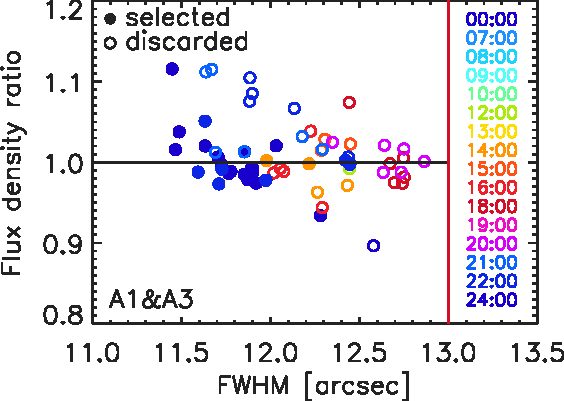
\includegraphics[clip=true, trim={0, -0.3cm, -0.3cm, 0}, width=0.525\linewidth]{Figures/plot_flux_density_ratio_fwhm_uranus_corrected_skydip_narrow_1mm.pdf}
%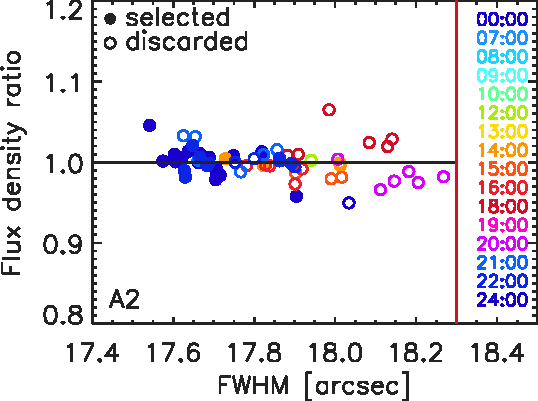
\includegraphics[clip=true, trim={0.7cm, -0.3cm, -0.25cm, 0}, width=0.465\linewidth]{Figures/plot_flux_density_ratio_fwhm_uranus_corrected_skydip_narrow_a2.pdf}
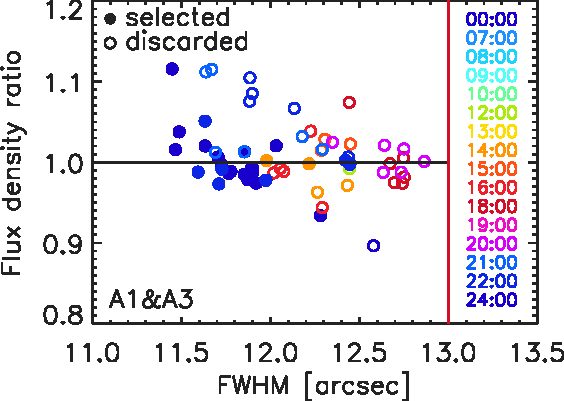
\includegraphics[clip=true, trim={0, -0.3cm, -0.3cm, 0}, width=0.72\linewidth]{Figures/plot_flux_density_ratio_fwhm_uranus_corrected_skydip_narrow_1mm.pdf}
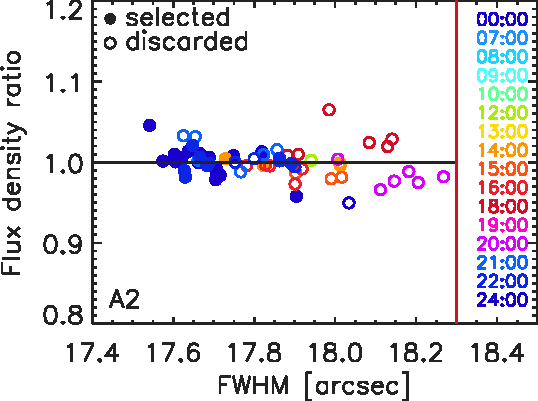
\includegraphics[clip=true, trim={0cm, -0.3cm, -0.6cm, 0}, width=0.707\linewidth]{Figures/plot_flux_density_ratio_fwhm_uranus_corrected_skydip_narrow_a2.pdf}
  
\caption[Uranus flux density stability against FWHM]{ Uranus flux
density ratio vs beam size after baseline calibration. The ratio
of Uranus measured flux densities to expectations as a function of the
measured 2D Gaussian beam FWHM is shown for the $1$-mm array
combination (top panel) and for array 2 (bottom panel) after absolute calibration using the
\emph{baseline} method. These plots include all Uranus scans acquired during the 
N2R9, N2R12 and N2R14 campaigns and whose beam FWHMs are below the threshold indicated
by the vertical red lines (open circles), as well as the scans that
met the \emph{baseline} selection criteria (filled circles).}
\label{fig:calib_uranus_vs_fwhm_all}
\end{center}
\end{figure}

The flux density estimates have been calibrated beforehands, so that
the flux density ratios are equal to unity in average by construction.
We observe no significant dependence of the selected scan flux ratios
(shown as filled circles in Fig.~\ref{fig:calib_uranus_vs_fwhm_all})
on the beam FWHM. {\lp This gives a first indication of the efficiency
  of the \emph{baseline} scan selection to mitigate the
temperature-induced beam variation effect. The flux stability against
the beam FWHM is further assessed in Sect.~\ref{se:photometry}.}


\subsubsection{Flux stability against the atmospheric transmission}
\label{se:baseline_calibration_atm}

We test the stability of Uranus flux densities calibrated using the
\emph{baseline} method against the atmospheric transmission. The latter
depends on the measured zenith opacity $\taunu$ and the scan
average \airmass\ x as $\exp{(-\taunu \, x)}$. In
the first row of Fig.~\ref{fig:calib_uranus_vs_atmtrans}, Uranus flux ratio
is shown as a function of the atmospheric
transmission for the $1$-mm array combination and Array 2 and for the
three \emph{reference} observation campaigns (N2R9, N2R12 $\&$ N2R14). We
observe no sizable correlation of the flux ratio with the atmospheric
transmission, which gives a first
indication of the robustness of the flux density estimates against the
atmospheric conditions using the baseline calibration. This will be
further tested using a larger number of scans toward other sources in
Sect.~\ref{se:photometry}.
%
\begin{figure}[!htbp]
\begin{center}
  % corrected skydip
  \begin{overpic}[clip=true, trim={0, -0.3cm, -0.3cm, 0}, width=0.49\linewidth]{Figures/plot_flux_density_ratio_obstau_uranus_corrected_skydip_narrow_1mm.pdf}
    \put(20,23){\footnotesize Baseline}
  \end{overpic}
  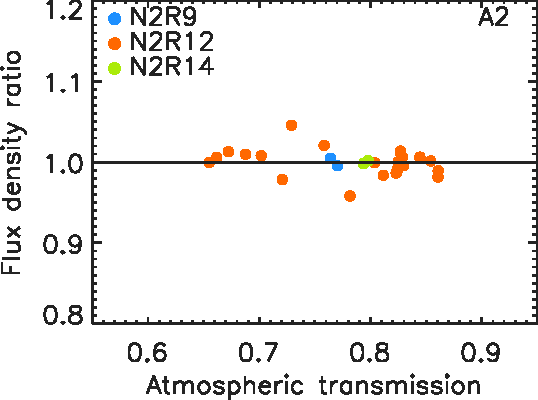
\includegraphics[clip=true, trim={0, -0.3cm, -0.3cm, 0}, width=0.49\linewidth]{Figures/plot_flux_density_ratio_obstau_uranus_corrected_skydip_narrow_a2.pdf}
  % taumeter
  \begin{overpic}[clip=true, trim={0, -0.3cm, -0.3cm, 0}, width=0.49\linewidth]{Figures/plot_flux_density_ratio_obstau_uranus_tau225_narrow_1mm.pdf}
    \put(20,23){\footnotesize Taumeter}
  \end{overpic}
  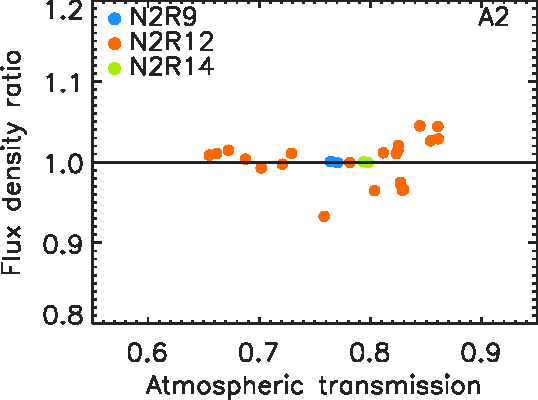
\includegraphics[clip=true, trim={0, -0.3cm, -0.3cm, 0}, width=0.49\linewidth]{Figures/plot_flux_density_ratio_obstau_uranus_tau225_narrow_a2.pdf}
  % skydip
  \begin{overpic}[clip=true, trim={0, -0.3cm, -0.3cm, 0}, width=0.49\linewidth]{Figures/plot_flux_density_ratio_obstau_uranus_skydip_narrow_1mm.pdf}
    \put(20,23){\footnotesize Skydip}
  \end{overpic}
  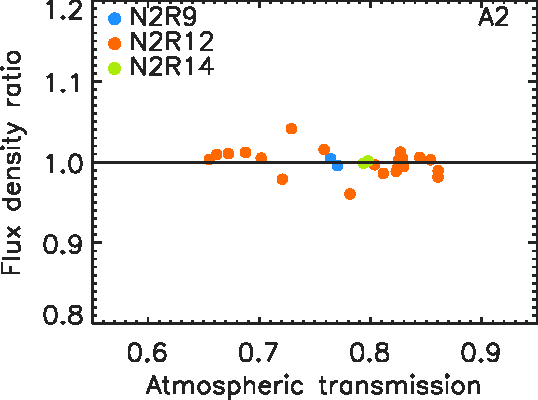
\includegraphics[clip=true, trim={0, -0.3cm, -0.3cm, 0}, width=0.49\linewidth]{Figures/plot_flux_density_ratio_obstau_uranus_skydip_narrow_a2.pdf}
  \caption[Uranus flux density stability against atmospheric
    transmission]{Uranus flux density ratio vs atmospheric transmission
    shown for the $1$-mm array
    combination (left column) and for array 2 (right column) after absolute
    calibration using (\emph{first row}) the baseline method, (\emph{second row}) the 'taumeter'-based and
    (\emph{third row}) the 'skydip'-based methods. These plots
    include all Uranus scans acquired during N2R9, N2R12 and N2R14
    campaigns. }
  \label{fig:calib_uranus_vs_atmtrans}
\end{center}
\end{figure}
%


\subsubsection{Comparison with other opacity correction methods}
\label{se:baseline_calibration_opacity}

As a cross-check we have derived the absolute
calibration factors using the {\tt taumeter}
(Sect.~\ref{se:taumeter-method}) and the {\tt skydip}
(Sect.~\ref{se:skydip-method}) atmospheric opacity
correction methods. We then compare Uranus
flux density estimates after absolute calibration using the baseline
calibration and these two alternative corrections. Figure~\ref{fig:calib_uranus_vs_atmtrans}
shows the Uranus measured-to-modeled
flux ratio as a function of the atmospheric transmission for A1$\&$A3
and for A2 after the {\tt taumeter} correction (second row) and
after the {\tt skydip} correction (third row). We observe more
dispersion for the {\tt taumeter}-based flux ratio, whereas the {\tt
skydip}-based ratio is very similar as the baseline ratio except
for a slight decrease of the flux at low atmospheric
transmission. Thus the {\tt taumeter} and {\tt skydip} atmospheric
opacity correction methods can be used for
the absolute calibration in complement to {\tt corrected skydip}, e.g. to
perform robustness tests as in Sect.~\ref{se:photometry}. 



%---------------------------------------------------------------------
%	PHOTOMETRIC CORRECTION
%---------------------------------------------------------------------
\subsection{Photometric correction}
\label{se:photometric_correction}

The \emph{baseline} calibration (Sect.~\ref{se:baseline_calibration}) relies
on the \emph{baseline} scan selection, as defined in Sect.~\ref{se:data_selection}, to
mitigate the \afternoon\ beam size variations, which is discussed in
Sect.~\ref{se:beam_variation}. By contrast, in this section, we
address the issue of calibrating even during the observing periods
impacted by the \afternoon\ beam variation effect. We discuss an
alternative calibration method that
relies on a photometric correction depending on the beam size.
{\lp The key idea is to perform a joint monitoring of flux estimates
  using the fixed-width Gaussian amplitude and of the beam size.}
The objective is both to cross-check the baseline calibration results
using more observation scans and to anticipate on future developments
that could be deployed if an accurate beam monitoring is performed.


\subsubsection{Photometric correction method}
\label{se:photometric_correction_method}

When the beam size broadens due to e.g. \afternoon\ beam effect, the
flux density is smeared in a larger solid angle and
the flux density estimator, which is based on the amplitude fit of a
Gaussian beam of fixed FWHM (see
Sect.~\ref{se:photometric_system}) is biased toward low flux
densities.

Considering only the main beam broadening, modeled as a Gaussian of
size $FWHM' = 2 \sqrt{2\ln{2}} \, \sigma '$, we show in
Appendix~\ref{ap:photometric_correction_detail} that
the flux density estimator depends on {\lp $(\sigma'^2 +\sigma_0^2)$
  that is the squared size of the Gaussian
  resulting from the convolution} between the enlarged
$\sigma '$-Gaussian, which can be monitored as in Sect.~\ref{se:beam_variation}, and the 
$\sigma_0$ fixed-width Gaussian of our reference system.

An unbiased
flux density $\hat{S}_{\rm{pc}}$ can be derived from the flux density
estimate $\hat{S}$ as
\begin{equation}
  \hat{S}_{\rm{pc}} = f(\sigma')\, \hat{S},
\end{equation}
where $f(\sigma')$ is a photometric correction for the beam variation
effect. Within the Gaussian model, it reads:
\begin{equation}
  f(\sigma') = \frac{(\sigma'^2 + \sigma_0^2)}{(\sigma_{\star}^2 + \sigma_0^2)}. 
\end{equation} 

The beam size in stable atmospheric condition $\sigma_\star$ is
determined by measuring the 2D Gaussian beam on the series of scans of
source with varying flux densities, which have been used for the beam
characterization in Sect.~\ref{se:mainbeam}. However, $\sigma_\star$
is not equivalent to the main beam Gaussian size since the side lobes
and first error beams are not masked for the beam size
monitoring. The $\sigma_\star$ estimates are slightly
larger {\lp for bright sources due to the contribution of the first side
lobes and error beams, which is above the noise level, in the Gaussian fit.}  
%for sources bright enough for the side lobes to be well above
%the noise level.
An empirical model for the induced correlation of
$\sigma_\star$ with the source flux density is given in
Appendix~\ref{ap:photometric_correction_detail}.

The photometric correction thus relies on the measure of the current beam
size $\sigma'$. The induced uncertainties on the flux density
measurements depend on the precision of which we are able to monitor
the beam size. We perform two case studies, which correspond to the
two beam monitoring methods discussed in
Sect.~\ref{se:beam_variation}.\\
%\new{the paragraph titled ``Demonstration case''} presents a demonstration
%calibration assuming the beam is precisely monitored, whereas
%the ``Practical case using pointing scans'' paragraph addresses a practical calibration relying
%on a beam monitoring using pointing scans. 

\noindent \emph{Demonstration case} This method, shortened as {\tt PC-demo}
hereafter, uses a photometric correction based on the beam monitoring
with bright source scans. Both the 2D Gaussian FWHM fit and the
FWHM$_0$ photometry are performed on the map of the
source. This method thus applies only on point-like
sources that are bright enough for an accurate fit of the beam to be
obtained using a single scan.

To capture only the beam size variations driven by the
observing conditions (primary mirror deformations, anomalous
refraction, elevation), a small correction $\delta_{\rm{FWHM}}$ has to be made to
the 2D Gaussian beam FWHM estimate for bright sources. The estimate of the
actual Gaussian size $\sigma '$ is
% ATTENTION SIGMA GEOM PAS DEFINI
\begin{equation}
  \hat{\sigma '} = \frac{(\rm{FWHM} - \delta_{\rm{FWHM}})}{2\sqrt{2 \ln{2}}}, 
\end{equation} 
where the offset $\delta_{\rm{FWHM}}$ is null for faint or moderately
bright point sources, and non-zero for bright sources.
As for $\sigma_\star$, the 2D Gaussian fit yields slightly broaden
%$\sigma_{\rm{geom}}$
FWHM for bright sources (e.g. planets) to accomodate
for the side lobes and error beams, which are measured with high signal-to-noise.
For Uranus, $\delta_{\rm{FWHM}}$ includes also the beam widening due
to Uranus disc, as discussed in Sect.~\ref{se:mainbeam_results}.
%, which is seen with an average diameter of $3.5''$ at the
%IRAM 30-m telescope latitude.
We measure Uranus $\delta_{\rm{FWHM}}$
by comparing the average %$\sigma_{\rm{geom}}$
FWHM estimates using Uranus
scans and using MWC349 scans, we found $\delta_{\rm{FWHM}} = 0.4''$ at
1\,mm and $\delta_{\rm{FWHM}} = 0.25''$ at 2\,mm, which basically
distributes as one half being due to Uranus finite extension and the
other half stemming from the side lobes.\\

\noindent \emph{Practical case using pointing scans} This method,
shortened as {\tt PC-point} hereafter, performs a photometric correction
based on the beam monitoring with pointing scans. Unlike
{\tt PC-demo}, this method is thus usable even for sources fainter
than about one Jy. The Gaussian beam size $\sigma '$ is estimated
using the beam size estimate interpolated from the pointing-based beam
monitoring. {\lp For Uranus, this value is corrected for the diameter
size, as in Sect.~\ref{se:mainbeam_results}.}  
%The actual Gaussian beam size $\sigma '$ is estimated using
%\begin{equation}
%  \hat{\sigma '} = \sigma_{\rm{p}} - \frac{\delta_{\rm{p}}}{2\sqrt{2 \ln{2}}}, 
%\end{equation} 
%where $\sigma_{\rm{p}}$ is the beam size estimate interpolated from
%the pointing-based beam monitoring and the offset $\delta_{\rm{p}}$
%only accounts for the source finite extension. It is null for
%point-like sources and equals to $0.2''$ at $1\,\rm{mm}$ and $0.13''$
%at $2\,\rm{mm}$ for pointing scan of Uranus.
%No other contribution
%enters $\delta_{\rm{p}}$
No other FWHM offset correction is needed since pointing scan maps
have a low signal-to-noise ratio that prevents the geometrical FWHM
from being significantly affected by the side lobes.


%%%%%%%%%%%%%%%%%%%%%%%%%%%%%%%%%%%%%%%%%%%%%%%%%%%%%%%%%%%%%%%%%%%
%    Flux ratio vs FWHM
\begin{figure}[!htbp]
  \begin{center}
    % corr. sky. photocorr demo
    \begin{overpic}[clip=true, trim={0, -0.3cm, -0.3cm, 0},width=0.525\linewidth]{Figures/plot_flux_density_ratio_fwhm_uranus_corrected_skydip_photocorr_demo_narrow_1mm.pdf}
       \put(18,25){\footnotesize PC-demo}
    \end{overpic}
    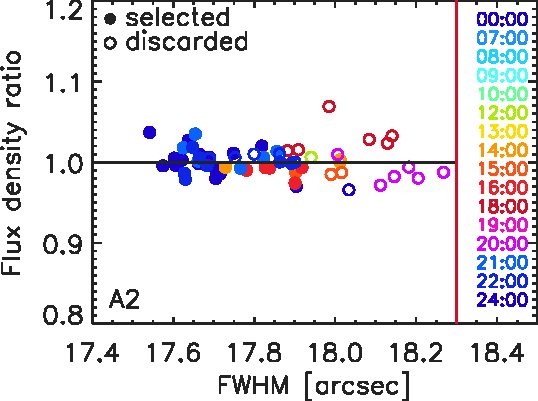
\includegraphics[clip=true, trim={0.7cm, -0.3cm, -0.25cm, 0}, width=0.465\linewidth]{Figures/plot_flux_density_ratio_fwhm_uranus_corrected_skydip_photocorr_demo_narrow_a2.pdf}
    % corr. sky. photocorr pointing
    \begin{overpic}[clip=true, trim={0, -0.3cm, -0.3cm, 0},width=0.525\linewidth]{Figures/plot_flux_density_ratio_fwhm_uranus_corrected_skydip_photocorr_pointing_narrow_1mm.pdf}
      \put(18,25){\footnotesize PC-point}
    \end{overpic}
    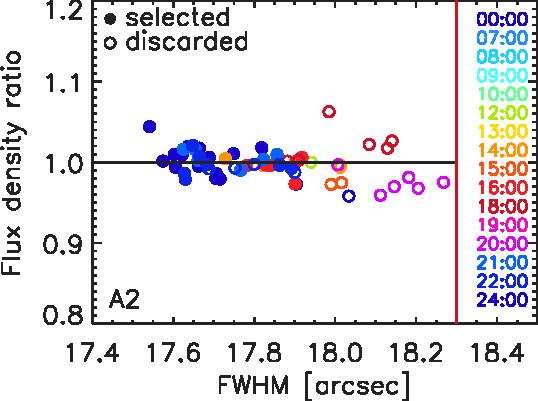
\includegraphics[clip=true, trim={0.7cm, -0.3cm, -0.25cm, 0}, width=0.465\linewidth]{Figures/plot_flux_density_ratio_fwhm_uranus_corrected_skydip_photocorr_pointing_narrow_a2.pdf}
    \vspace{-0.5cm}
    \caption[Uranus flux density stability against FWHM]{
      \small{Uranus flux density ratio vs beam size for calibration
  with photometric correction. The ratio of 
      Uranus measured flux densities to expectations as a function of the
      measured 2D Gaussian beam FWHM is shown for the $1$-mm array
      combination (left column) and for array 2 (right column) after absolute
      calibration using (\emph{first row}) the {\tt PC-demo} and (\emph{second
        row}) the {\tt PC-point} photometric corrections. These plots
      include all Uranus scans acquired during N2R9, N2R12 and N2R14
      campaigns and whose beam FWHMs are below the threshold indicated
      by the vertical red lines, (open circles), as
      well as the scans that met the baseline scan selection criteria (filled
      circles).}}
\label{fig:calib_uranus_vs_fwhm_photocorr}
\end{center}
\end{figure}

\subsubsection{Absolute calibration with a photometric correction}

We perform the absolute calibration by i) implementing the practical
method described in Sect.~\ref{se:practical_calib}, ii) correcting the
atmospheric attenuation using the {\tt corrected skydip} opacity
estimates, and iii) using the photometric correction of
Sect.~\ref{se:photometric_correction_method}.

Using the photometric correction alleviates the need of
performing a scan selection based on the observation time. However,
the scans from which the absolute calibration is derived, are selected
on the FWHM estimate using the same criteria as for the baseline
calibration, that are FWHM thresholds of $12.5''$ at $1\, \rm{mm}$ and $18''$ at
$2\, \rm{mm}$. Thus, only the scans that are moderately affected by the beam
effect are included in the absolute calibration in order not to
include twice the photometric correction uncertainties in the error
budget (once for the absolute calibration and once for the photometry).

Figure~\ref{fig:calib_uranus_vs_fwhm_photocorr} presents the Uranus
measured-to-predicted flux density ratio as a function of the beam FWHM
after the photometric correction with the {\tt PC-demo} and
{\tt PC-point} methods. The flux
density is stable against the beam FWHM within uncertainties for both
wavelengths.

% ALL METHOD RESULTS 
\begin{table}[!htbp]
\caption[Comparison of calibration results using five methods]{Comparison of absolute calibration results using five methods}
\label{tab:Abs_calibration_results_all}
\centering
\begin{tabular}{clrrrrr}
  \hline\hline
  \noalign{\smallskip}
%  \multicolumn{2}{c}{}  &  \multicolumn{5}{|c|}{Methods} \\\cline{3-7}
  \multicolumn{2}{c}{}  &  baseline  & TM\tablefootmark{a}  &  SD\tablefootmark{b} & PC-d\tablefootmark{c} & PC-p\tablefootmark{d}  \\
  \noalign{\smallskip}
  \hline\hline
   \multicolumn{2}{c}{$\#$ scans} & 26    &       26  &    26    &    38           &    38 \\ 
  \hline
  \noalign{\smallskip}
%  Factor &  A1          &   1.00  &  0.97   &  1.13    &   1.01    &   1.02  \\
%         &  A3          &   1.00  &  0.97   &  1.02    &   1.01    &   1.00  \\
   Ratio  &  1mm         &   1.00  &  0.95   &  1.06    &   1.01    &   1.01  \\
          &  2mm         &   1.00  &  0.94   &  0.99    &   1.01    &   1.01  \\
  \hline
  \noalign{\smallskip}
%  RMS  &  A1            &  3.2    &   4.2   &   3.4    &    3.5    &   3.0 \\
%  $[\%]$     &  A3      &  3.6    &   4.3   &   3.3    &    3.5    &   3.0 \\
   RMS    &  1mm           &  3.3    &   4.5   &   3.3    &    3.1    &   2.6 \\
   $[\%]$ &  2mm           &  1.6    &   2.6   &   1.5    &    1.5    &   1.5 \\
\hline
\end{tabular}
\tablefoot{ Results based on 
    \tablefoottext{a}{the {\tt Taumeter} opacity correction}
    \tablefoottext{b}{the {\tt Skydip} opacity correction}
    \tablefoottext{c}{the {\tt PC-demo} photometry correction}
    \tablefoottext{d}{the {\tt PC-point} photometry correction}
    }
\end{table}

We further quantify the
difference between all the calibration methods that have been tested
in evaluating i) the average absolute calibration factor
with respect to the baseline calibration factor and
ii) the rms dispersion of the measured-to-modeled flux ratios. These
quantities are gathered in Table~\ref{tab:Abs_calibration_results_all}
in the rows labeled 'Ratio' and 'RMS' respectively. 

We find that, resorting to a photometric correction i) allows us to use $45\%$ more
scans for the absolute calibration, ii) has a negligible impact on
the absolute calibration factor and iii) yields a small reduction of
the flux density ratio dispersion. For the absolute calibration, the
{\tt PC-point} method performs as well as the {\tt PC-demo} one.
Photometry capability and stability when using a photometric
correction will be further tested in Sect.~\ref{se:photometry}. 
